\chapter{Overview of the {\XACC} Model and Language}
\label{chap: overview}

\section{Hardware Model}

The target of {\XMP} is distributed-memory multicomputers (Figure
\ref{fig1}). Each computation node, which may contain several cores, has
its own local memory (shared by the cores, if any), and is connected
with each other via an interconnection network.
%
Each node can access its local memory directly and remote memory, that
is, the memory of another node indirectly (i.e. via
communication). However, it is assumed that accessing remote memory is 
much slower than accessing local memory.

\begin{myfigure}
\includegraphics[width=12cm]{figs/Fig1.eps}
  \caption{Hardware Model}\label{fig1}
\end{myfigure}

\section{Execution Model}

The {\XMP} runtime system creates a team of threads on each node
when starting the user program execution. This team of threads is
composed by a single master thread and serveral additional worker
threads.

An {\XMP} program execution is based on the Single Program
Multiple Data (SPMD) model, where the master thread on each node
starts execution from the same main routine and keeps executing the
same code independently (i.e. asynchronously), as if an implicit
tasklet region encloses the whole program, until it encounters an
{\XMP} construct.

The set of nodes on each of which a thread executes a procedure, a
statement, a loop, a block, etc. is referred to as its {\it
\Term{executing node set}} and determined by the innermost {\tt task},
{\tt loop}, or {\tt array} directive surrounding it dynamically, or at
runtime.

The {\it \Term{current executing node set}} is the executing node set
for the current context, which is managed by the {\XMP} runtime system
on each node. The current node set at the beginning of the program
execution, or {\it \Term{primary node set}}, is a node set that contains
all the available nodes, which can be specified in an
implementation-dependent way (e.g. through a command-line option).

When a thread encounters at runtime either a {\tt loop}, {\tt array}, or
{\tt task} construct, and is executed on a node in the node set
specified by the {\tt on} clause of the directive, it updates the
current node set with the specified one and executes the body of the
construct, after which it resumes the last executing node set and
proceeds to execute the following statements.

Particularly when a thread encounters a {\tt loop} or an {\tt array}
construct, it executes the loop body or the array assignment in parallel
with threads on other nodes, so that each iteration of the loop or each
element of the assignment is independently executed on the node where
the specified data element resides.

When a thread encounters a synchronization or a communication
directive, synchronization or communication might occur between it and
threads on other nodes. That is, such {\it \Term{global constructs}}
should be performed collectively on the current nodes. Note that neither
synchronizations nor communications occur without these constructs
specified.

When a thread encounters a tasklet or a taskletloop construct, a new
tasklet is generated on the node. Execution of explicitly generated
tasklets is assigned to one of the threads on the node, subject to the
thread’s availability to execute work. Thus, execution of the new
tasklet could be immediate, or deferred until later according to
tasklet scheduling constraints and thread availability. Threads are 
allowed to suspend the current tasklet region at a tasklet scheduling
point in order to execute a different tasklet. If the suspended
tasklet region is for a tied tasklet, the initially assigned thread
later resumes execution of the suspended tasklet region. If the
suspended tasklet region is for an untied tasklet, then any thread may
resume its execution.


\section{Data Model}

%By default, data declared in the program are allocated in each node and
%are referenced locally by threads executed in the node. 

There are two classes of data in {\XMP}: {\it \Term{global data}} and
{\it \Term{local data}}. Data declared in an {\XMP} program are local by
default.

Global data are ones that are distributed onto the executing node set by
the {\tt align} directive (see section \ref{sub:align}). Each fragment
of a global data is allocated in the local memory of a node in the
executing node set.
%
%Note that the ``address'' of a global data is defined as that of its
%local section in each node and the results of any operations on such
%address are undefined.
%
%In contrast to a local-view programming model, a global-view programming
%model is a model in which programmers express their algorithm and data
%structure in their entirety, mapping them to the node set. The
%programmers describe the data distribution and the work mapping in order
%to express how to distribute data and share the workload among
%nodes. The variables in the global-view programming model appear as a
%shared memory spanning the nodes.

Local data are all of the ones that are not global. They are replicated
in the local memory of each of the executing nodes.

%{\XMP} supports two models of data viewing: the global-view programming
%model and the local-view programming model. In the local-view
%programming model, accesses to data in remote nodes are performed
%explicitly by language extension for get/put operations on remote nodes
%with the node number of the target nodes, while reference to local data
%is executed implicitly.

A node can access directly only local data and sections of global data
that are allocated in its local memory.
%
To access data in remote memory, explicit communication must be
specified in such ways as the global communication constructs and
the coarray assignments.

%\underline{Description on memory layout to be added.}

Particularly in {\XMPF}, for common blocks that include any global
variables, the ways how the storage sequence of them is defined and how
the storage association of them is resolved are
implementation-dependent.

% \section{Global-view Programming Model}

% The global-view programming model is useful when, starting from a
% sequential version of a program, the programmer parallelizes it in
% data-parallel style by adding directives with minimum modification.
% %
% In the global-view programming model, the programmer describes the
% distribution of the data among nodes using the data distribution
% directives.
% %
% The {\tt loop} construct assigns each iteration of a loop to the node
% where the computed data is located. 
% %
% The global-view communication directives are used to synchronize nodes,
% to maintain the consistency of the shadow area, and to move part of the
% distributed data globally.
% %
% Note that the programmer must specify explicitly communications to make
% all data reference in the program local by using appropriate directives.
% %Note that the programmer must perform all computations that require data
% %reference locally by any appropriate directives.

% In many cases, the {\XMP} program according to the global-view
% programming model is based on a sequential program and can produce the
% same results as it, regardless of the number of nodes (Figure
% \ref{fig2}).
% %The global view provides a 
% %programming model in which computation and data are distributed onto
% %computation nodes.

% There are three groups of directives for the global-view programming
% model. Since these directives are ignored as a comment by the
% compilers of base languages ({\Fort} and {\C}), an {\XMP} program can be
% compiled by them to run properly.

% %an  {\XMP} program derived from a sequential program can preserve the
% %integrity of the original program when the program is run sequentially. 

% \subsubsection*{Data Mapping}

% Specifies the data distribution and mapping to nodes (partially
% inherited from HPF).

% \subsubsection*{Work Mapping (Parallelization)}

% Assigns a work to a node set. The {\tt loop} construct maps each
% iteration of a loop to nodes owning a specified data elements. The {\tt
% task} construct defines an amount of work as a {\it \Term{task}} and
% assigns it to a specified node set.

% \subsubsection*{Communication and Synchronization}

% Specifies how to communicate and synchronize with the other compute
% nodes. In {\XMP}, inter-node communication must be explicitly specified
% by the programmer. The compiler guarantees that no communication occurs
% unless it is explicitly specified by the programmer.

% \begin{myfigure}
% \includegraphics[width=12cm]{figs/Fig2.eps}
%   \caption{Parallelization by the Global-view Programming Model}
% \label{fig2}
% \end{myfigure}

% \section{Local-view Programming Model}

% The local-view programming model is suitable for programs that
% explicitly describe an algorithm and remote data reference that are to
% be done by each node (Figure \ref{fig3}).
% %Since MPI is based on the local-view model, the local-view programming
% %model of {\XMP} has high interoperability with MPI.

% For the local-view programming model, some language extensions and 
% directives are provided. The coarray notation imported from {\Fort} 2008
% is one of such extensions and can be used to specify which replica of a
% local data is to be accessed. For example, the expression of {\tt
% A(i)[N]} is used to access an array element of {\tt A(i)} located on the
% node {\tt N}.
% %
% If the access is a reference, then communication to obtain the value
% from remote memory (i.e. {\it get} operation) occurs. If the access is a
% definition, then communication to set a value to remote memory
% (i.e. {\it put} operation) occurs.

% \begin{myfigure}
% \includegraphics[width=12cm]{figs/Fig3.eps}
%   \caption{Local-view Programming Model}
% \label{fig3}
% \end{myfigure}

% \section{Interactions between the Global View and the Local View}

% In the global view, nodes are used to distribute data and computational
% load. In the local view, nodes are used to address data in the coarray
% notation.
% %
% In the application program,
% programmers should choose an appropriate data model according to the
% structure of the program. Figure \ref{fig4} illustrates the global view
% and the local view of data.

% Data may have both a global view and a local view, and can be accessed
% from either. {\XMP} provides some directives to give the local name
% (alias) to the global data declared in the global-view programming model
% so that they can be accessed also in the local-view programming
% model. This feature is useful to optimize a certain part of the program
% by using explicit remote data access in the local-view programming
% model.

% \begin{myfigure}
% 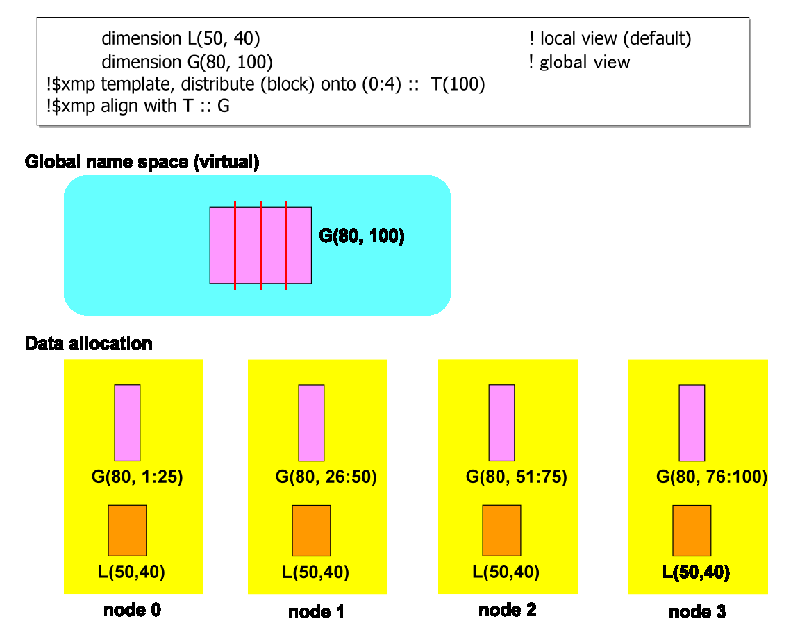
\includegraphics[width=12cm]{figs/Fig4.eps}
%   \caption{Global View and Local View}
% \label{fig4}
% \end{myfigure}

% \section{Base Languages}

% The XcalableMP language specification is defined on Fortran or C as a
% base language. More specifically, the base language of XcalableMP
% Fortran is Fortran 90 or later, and that of XcalableMP C is ISO C90
% (ANSI C89) or later.
